\documentclass[12pt]{article}
\usepackage{amsmath, amssymb, geometry, fancyhdr}
\usepackage{MnSymbol,wasysym}
\geometry{a4paper, margin=1in}
\setlength{\headheight}{15pt}
\pagestyle{fancy}
\fancyhf{}
\fancyhead[L]{CSCI-769 Quantum Computing Principles and Applications}
\fancyhead[R]{}
\fancyfoot[C]{\thepage}
\newcommand{\bra}[1]{\langle #1 |}
\newcommand{\ket}[1]{| #1 \rangle}
\usepackage{xcolor}
\usepackage{hyperref}
\usepackage{piton}
\usepackage{quantikz}
\usepackage{listings}

\lstset{
    language=Python,
    basicstyle=\ttfamily\small,
    keywordstyle=\color{blue},
    commentstyle=\color{green},
    stringstyle=\color{red},
    numbers=left,
    numberstyle=\tiny\color{gray},
    frame=single,
    breaklines=true,
    captionpos=b
}

\begin{document}

\title{CSCI-769 Quantum Computing Principles and Applications Homework 3}
\author{}
\date{}
\maketitle

\subsection*{1) Quantum Repetition Code In Qiskit in Ideal Circumstances (20 pts)}
\textbf{Summary}: In this problem my goal is to show you how quantum repetition code works, and its ability to correct errors with the Qiskit Simulator in an ideal situation. We will based on a coin flip produce a state $\ket{000}$ or $\ket{100}$ based on if an $X$ gate is applied to the first qubit or not. In the ideal situation, under this assumption, we should always measure $\ket{000}$. Because the syndrome with either do nothing to the "good" $\ket{0}_{L} = \ket{000}$ state or flip the first bit back in $\ket{100}$ to $\ket{0}_{L} = \ket{000}$. We will see some interesting things here, team \smiley{}!
\begin{itemize}
    \item a) Make a circuit in Qiskit that randomly applies an X gate with probability $0.5$ to a $\ket{0}$ qubit, and measure. Run this circuit 100 times on a simulator, and report what you measure. This "flipping of the coin" will be seen as adding a bit flip error to our logical qubit eventually \smiley{}.
    \item (b) Consider the quantum repetition code below. Implement it (without the "error block"). The state $ \ket{\psi}$ is derived from randomly applying the X gate in part (a). Investigate which combinations of ancilla measurements through syndrome extraction and decoding correspond to correcting specific qubits with an X gate flip. Check the "c if" function in Qiskit to learn how to apply gates to certain qubits based on mid-circuit measurements to perform the "correct" block! Measure all the data qubits after the error correction is complete to determine what state is observed, and perform 100 shots on a simulator. Also report the asilla qubit measurements in a plot as well.
    \item  (c) Instead of one time of doing the error correction routine with anscillas, do it ten times. That is to say, do the part of the error correction and then measure the ansillas, then do that repeatedly, to collect and count the number of times you see particular syndromes from the ansillas. Then based on which syndrome is seen the most correct the qubit by a "majority vote rule" (since I am a fan of freedom and democracy team \smiley{}). Do this 100 times on a simulator and compare it with the previous part results. Also report the ancilla qubit measurements in a plot as well.
    

\end{itemize}
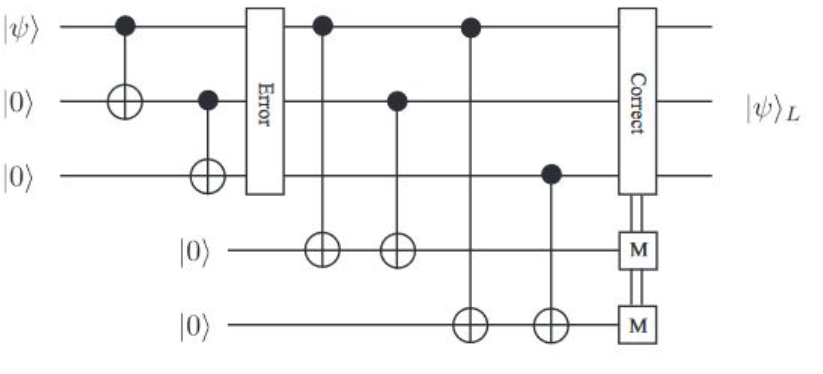
\includegraphics[scale=.5]{rep.png}

\subsection*{2) Quantum Repetition Code in Qiskit On A Real Machine (20 pts)}
\textbf{Summary:} The repetition code is meant to correct at most one bit flip error. Here we will explore its ability to do so on a real quantum machine.

a) Redo 1) but running it on an IBM NISQ, instead of 100 shots do 10. Describe your observations on doing this problem on a simulator versus NISQ. 

\subsection*{3) The Steane Code In Both an Ideal and Real World Machine (20 pts)}
Consider the Steane Code: 

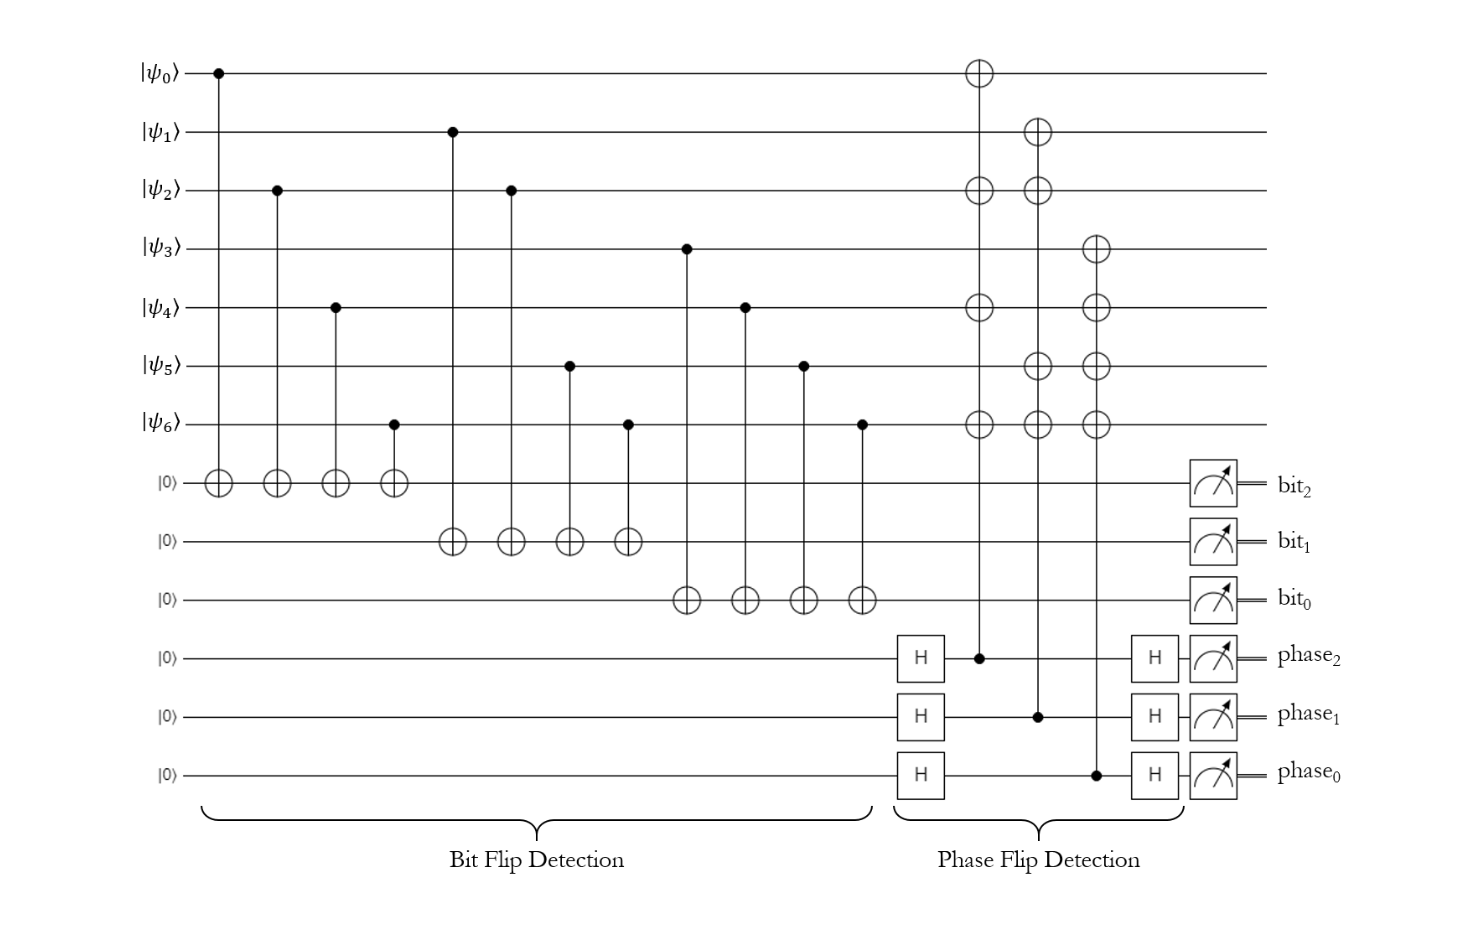
\includegraphics[scale=.4]{steane.png}

Redo the problems in 1) and 2) but with the Steane code, and a slight modification. In this case, we will be applying an X gate with probability $0.5$ to the second $\ket{0}$ qubit, but afterwards, also applying a Z gate with $0.5$ probability to the second. While in the measurements of the data qubits you will see you correct the flip, you cannot see a flip error was detected. From the  readout of the ancillas you will at least be able to see that the phase error was detected. But we cannot see if the phase error has been fixed, like a flip error, since we are in the standard basis. Maybe we'll redo this problem in the the Hadamard basis someday to observe the phase error has been corrected \smiley{}.
\subsection*{4) Logical Error Rate (20 pts)}
\textbf{Summary:} Logical qubits are the vechnical in which quantum computation is stable and scalable. While one has to have a lot of physical qubits to encode, we can achieve logical error rates small enough to support any algorithm of interest (theoretically). In this problem you will explore that practically. 
Consider a surface code used for quantum error correction, where the logical qubit is encoded using a grid of physical qubits. The parameters of the code are:

\begin{itemize}
    \item $d$: Code distance, which determines the number of errors the code can correct ($\lfloor (d-1)/2 \rfloor$ errors).
    \item $p$: Physical qubit error rate.
    \item $p_{\text{th}}$: Code threshold, below which increasing the distance $d$ suppresses the logical error rate.
    \item $p_L$: Logical error rate of the encoded qubit.
    \item $N_q$: Number of physical qubits required to encode a single logical qubit.
\end{itemize}

The number of physical data qubits needed to encode a logical qubit in a surface code is approximately:
\begin{equation}
    N_q \approx c d^2,
\end{equation}
where $c$ is a small overhead constant.

The logical error rate $p_L$ can be approximated as:
\begin{equation}
    p_L \approx A \left( \frac{p}{p_{\text{th}}} \right)^{\frac{d+1}{2}},
\end{equation}
where $A$ is a fitting constant.

\subsection*{Economic Relevance}
For quantum computing to be economically relevant, error rates would be many orders of magnitude smaller than can most likely be achieved for physical qubits. This leads to a notion of a more stable logical qubit, the logical error rate must be low enough to run useful quantum algorithms. Assume the following application requirements:

\begin{itemize}
    \item Simulating quantum materials and condensed matter physics: $p_L \leq 10^{-15}$.
    \item Quantum chemistry simulations for reaction dynamics: $p_L \leq 10^{-12}$.
    \item Optimization problems in machine learning and combinatorial optimization: $p_L \leq 10^{-9}$.
\end{itemize}

\begin{itemize}
    \item (a) Comment on the behavior of the logical error rate as $d \rightarrow \infty$ when $p > p_{\text{th}} $ and $p < p_{\text{th}}$. What does this mean practically for the logical error rate if we can drive the physical error rate below a given surface codes threshold? In theory, can we make the logical error rate arbitrarily small?
    \item (b) Estimate the physical qubit count $N_q$, code distance $d$, and number of errors that are able to be detected and fixed, assuming constants $A=1$ and $c=2$ for each application in all four combinations of:
\begin{enumerate}
    \item Physical qubit error rate $p \in \{10^{-3}, 10^{-4}\}$ (corresponding to a CNOT gate error rate - usually the worst performing gate).
    \item Code threshold $p_{\text{th}} \in \{10^{-2}, 10^{-3}\}$ (this is typically surface code chosen dependent but represents a 1\% and .1 \% threshold respectively).
    
\end{enumerate}
    
\end{itemize}

\subsection*{5) Classical Versus Quantum Potential Error Size (20 pts)}
\textbf{Summary:} The different types of errors a qubit can experience compared to a classical bit have major implications for the complexity involved in performing error correction on a quantum computer versus a classical computer. In this problem, we will count how many potential combinations of error syndromes a classical bit can have for $q$ bits versus $q$ qubits. 
\begin{itemize}
    \item (a) For a single classical bit, either a bit can have an error or no error as a syndrome, which is two situations. If we have $q$ bits, how many syndromes can such a system potentially have?
    \item (b) Redo this analysis for a qubit, describing how many syndromes a single will admit. How many syndromes can a system of $q$ qubits have?
    \item (c) From (4), typically for an application $q=d^2$ data qubits (we encode that many qubits into a single logical state) and $d^2-1$ ancilla qubits. For this logical state, calculate the number of syndromes the qubit system can experience with an error rate of $10^{-3}$ and threshold of $10^{-2}$. This indicates of why quantum error correction is so much more involved and requires very complex decoding to figure out which qubit an error has occurred in, and how to fix said error. In classical bits, the only thing you have to do is keep track of bit flips (parity check). TL;DR Quantum Error Correction is exponentially harder than classical error correction, but will be vital for making quantum computers stable and scalable, team \smiley{}!!!
\end{itemize}





\subsection*{Bonus Problem: Realizing One And Two Qubit Gates On Hardware (50 pts)}
Recall we have many unitaries for realizing certain desired operations on quantum gates. For example consider an instance of a one and two qubit gate: 
% Requires: \usepackage{amsmath}
\begin{equation}
    X = 
    \begin{pmatrix}
        0 & 1 \\
        1 & 0
    \end{pmatrix}
\label{eq:x_matrix}
\end{equation}

% Requires: \usepackage{amsmath}
\begin{equation}
    \text{CNOT} = 
    \begin{pmatrix}
        1 & 0 & 0 & 0 \\
        0 & 1 & 0 & 0 \\
        0 & 0 & 0 & 1 \\
        0 & 0 & 1 & 0
    \end{pmatrix}.
\label{eq:cnot_matrix}
\end{equation}

We know what these operators do to one and two qubit systems. But how would a quantum computer actually implement these unitaries on a physical device? The answer is we will develop electromagnetic pulse sequences that we will send to the qubits! The application of a pulse sequence to a qubit will achieve the unitary operation we desire! This problem will help you begin to appreciate the mathematics (mainly optimization, and optimal control theory, needed to generate such pulses).

In QuTip find pulse sequences that realize both the X and CNOT gates respectively. I think this code will get you started - \href{https://github.com/qutip/qutip-notebooks/blob/master/examples/control-pulseoptim-Hadamard.ipynb}{example code for generating a pulse sequence for an $H$ gate}


For each gate, report the infidelity of the gate operation (the probability more or less of the gate failing to be realized from this pulse sequence), plot the control pulse sequence function found on the qubit(s), and plot all the quantum states probabilities as a function of time in both the one and two qubit examples from their potential starting states (2 plots for the X gate, and 4 for the CNOT gate). For example in the one qubit example plot the probability evolution for the $\ket{0}$ and $\ket{1}$ respectively, and for the two qubit problem plot $\ket{00}$, $\ket{01}$, $\ket{10}$, $\ket{11}$.

Explanation of $U_0$: this is the initial condition which is meant for the closed system considered that regardless of starting in the zero or one state (each column of this identity matrix) the pulse sequence will achieve the Hadamard transformation. For the two qubit example this would be a $4\times 4$ identity. This means each column of $U(t)$ represents the quantum state that has evolved from the initial column of $U_0$. So for example in the one qubit case - the first column is the evolution if you start in the zero state, and the second column is if you start in the one state. For the 2 qubit it then follow each column corresponds to $\ket{00}$, $\ket{01}$, $\ket{10}$, $\ket{11}$

Note: This is currently a closed system model, so you will notice quite low infidelities—perhaps $10^{-10}$ or smaller! This might confuse you, as I mentioned earlier that in the logical qubit example, the CNOT error rates are around $10^{-3}$. In open systems, it is probably going to be physically unlikely to achieve $10^{-10}$. In the next homework assignment, the bonus will involve generating pulse sequences for an open system, and you'll experience how those noises can significantly impact your infidelity compared to what you see here (it will get bigger by many orders of magnitude)! Stay tuned - Ryan is a man with a plan \smiley{}.

Hint: For the $X$ gate, just change the gate in the starter code, and figure out how to plot the probabilities over time \smiley{}

Hint 2: For the $CNOT$, this code and a bit of elbow grease, research, and some thought is all you need - there are multiple ways you can do it so you can even edit the code as well for a final solution, but keep the H\_d unchanged (you can mess around with different pulse shapes, etc, though):
\begin{lstlisting}
# Step 1: Define the System Hamiltonian
# Define Pauli matrices
sx = sigmax()
sy = sigmay()
sz = sigmaz()
I = identity(2)

# Parameters
omega = 1.0  # Qubit energy
J = 0.1      # Coupling strength

# Drift Hamiltonian (System's natural evolution)
H_d = (omega / 2) * (tensor(sz, I) + tensor(I, sz)) + J * (tensor(sx, sx) + tensor(sy, sy) + tensor(sz, sz))

# Control Hamiltonians (External fields)
H_c1 = tensor(sx, I)  # Control field on first qubit in x-direction
H_c2 = tensor(sy, I)  # Control field on first qubit in y-direction
H_c3 = tensor(I, sx)  # Control field on second qubit in x-direction
H_c4 = tensor(I, sy)  # Control field on second qubit in y-direction

H_controls = [H_c1, H_c2, H_c3, H_c4]

# Step 2: Define Time-Dependent Control Pulses
# Define time grid
tlist = np.linspace(0, 10, 100)  # Time evolution from 0 to 10 with 100 steps

# Example: Define control pulses (arbitrary pulse shapes)
def control_pulse1(t, args):
    return np.sin(t)  # Example: sinusoidal control field

def control_pulse2(t, args):
    return np.exp(-t)  # Example: exponentially decaying field

# Control field amplitudes (can be optimized later)
c1_coeff = [control_pulse1]
c2_coeff = [control_pulse2]
c3_coeff = [lambda t, args: 0.5 * np.sin(t)]  # Another example function
c4_coeff = [lambda t, args: 0.5 * np.exp(-t)]

# Step 3: Set Up the Time Evolution
# Define the Hamiltonian as a list with time-dependent components
H = [H_d, 
     [H_c1, c1_coeff], 
     [H_c2, c2_coeff], 
     [H_c3, c3_coeff], 
     [H_c4, c4_coeff]]

# Step 4: Solve the Schrödinger Equation
# Initial state (Example: |00⟩ state)
psi0 = tensor(basis(2, 0), basis(2, 0))

# Solve the Schrödinger equation
result = mesolve(H, psi0, tlist, [], [])

# Extract expectation values for analysis (e.g., probability of being in state |11⟩)
expectations = [result.states[i].dag() * tensor(basis(2, 1), basis(2, 1)) * result.states[i] for i in range(len(tlist))]

# Step 5: Optimize Control Pulses (Optional)
# Define optimization parameters
n_ts = 100  # Number of time slices
evo_time = 10  # Evolution time
fid_err_targ = 1e-4  # Target fidelity error

\end{lstlisting}

Hint 3: The optimize\_pulse function in qutip pulseoptim library might be useful!!!

\end{document}


\end{document}
